\section{Introduction}
\label{sec:introduction}

Many world action models (WAMs) produce predicted futures alongside robot actions \citep{kim2026cosmospolicy,nvidia2026cosmos3}. Joint generation, however, does not imply that action computation uses the predicted future: a policy could map the current observation and instruction directly to an action while producing a plausible future as an auxiliary output. Alternatively, predicted-future representations may serve as a computational workspace, encode a prospective robot pose for inverse dynamics \citep{hu2025vpp,du2023unipi}, or represent consequences used to evaluate actions \citep{ebert2018visualforesight,du2024videolanguage}.

RIFT provides the closest prior causal evidence by masking reads from and editing values at predicted-future positions in several WAMs \citep{zhang2026rift}. These interventions establish that behavior depends on information carried through the predicted-future interface. Because disrupting the interface can move an action in any direction, however, they do not reveal how a particular coherent future shapes behavior. We adapt mechanistic interventions to this joint video--action modality to make directional, testable claims about both future content and its computational pathway.

We ask three questions: Does coherent future content direct behavior; what visual content explains the effect; and which internal pathway carries it? In Stage 1, we insert one normal rollout's future representation into another rollout from the same saved state. The receiving rollout is the \emph{recipient}; the source is the \emph{donor}. We recompute the recipient's action while holding all other inputs fixed. The donor action is never shown to the model and serves only as a directional reference after inference. For Cosmos 3, Stage 2 keeps the donor future inserted but restores keys and values at predicted-future positions from the recipient's native run, testing how much of the Stage-1 effect passes through that interface.

The experiments yield three findings. First, Cosmos 3 donor futures redirect actions and executed endpoints almost completely toward the donor across 22 states and six tasks; Cosmos Policy shows a smaller early-state effect across all ten LIBERO-Long tasks. Second, Cosmos Policy's effect is concentrated in visual future targets, especially the wrist camera, whereas isolated robot or object pixels cannot reproduce Cosmos 3's complete-video effect. Third, restoring recipient K/V at predicted-future positions removes 83--88\% of mean Cosmos 3 steering, with a positive reduction in all 22 tested states. Together, the interventions support two concrete claims: coherent donor futures predict the direction of action changes, and future-token K/V carries most of that change in Cosmos 3.

\paragraph{Related work.}
Visual robot policies may infer actions from predicted video, condition on its representation, or generate futures and controls jointly \citep{du2023unipi,hu2025vpp,guo2024pad,li2025uva,kim2026cosmospolicy,nvidia2026cosmos3,ye2026dreamzero}. These objectives do not establish how a particular future participates in inference. Recent work tests whether explicit rollout is needed \citep{li2025uva,yuan2026fastwam}, aligns foresight and action representations \citep{qiu2026agra}, or intervenes on predicted-future positions \citep{zhang2026rift}. Activation and path patching test whether a representation or route affects output \citep{vig2020causalmediation,meng2022rome,goldowskydill2023pathpatching}. We use coherent within-state counterfactuals and a directional metric to identify the effect carried through predicted-future K/V \citep{zhang2024activationpatching}.

\section{Two-Stage Intervention Design}
\label{sec:methods}

\begin{figure*}[t]
  \centering
  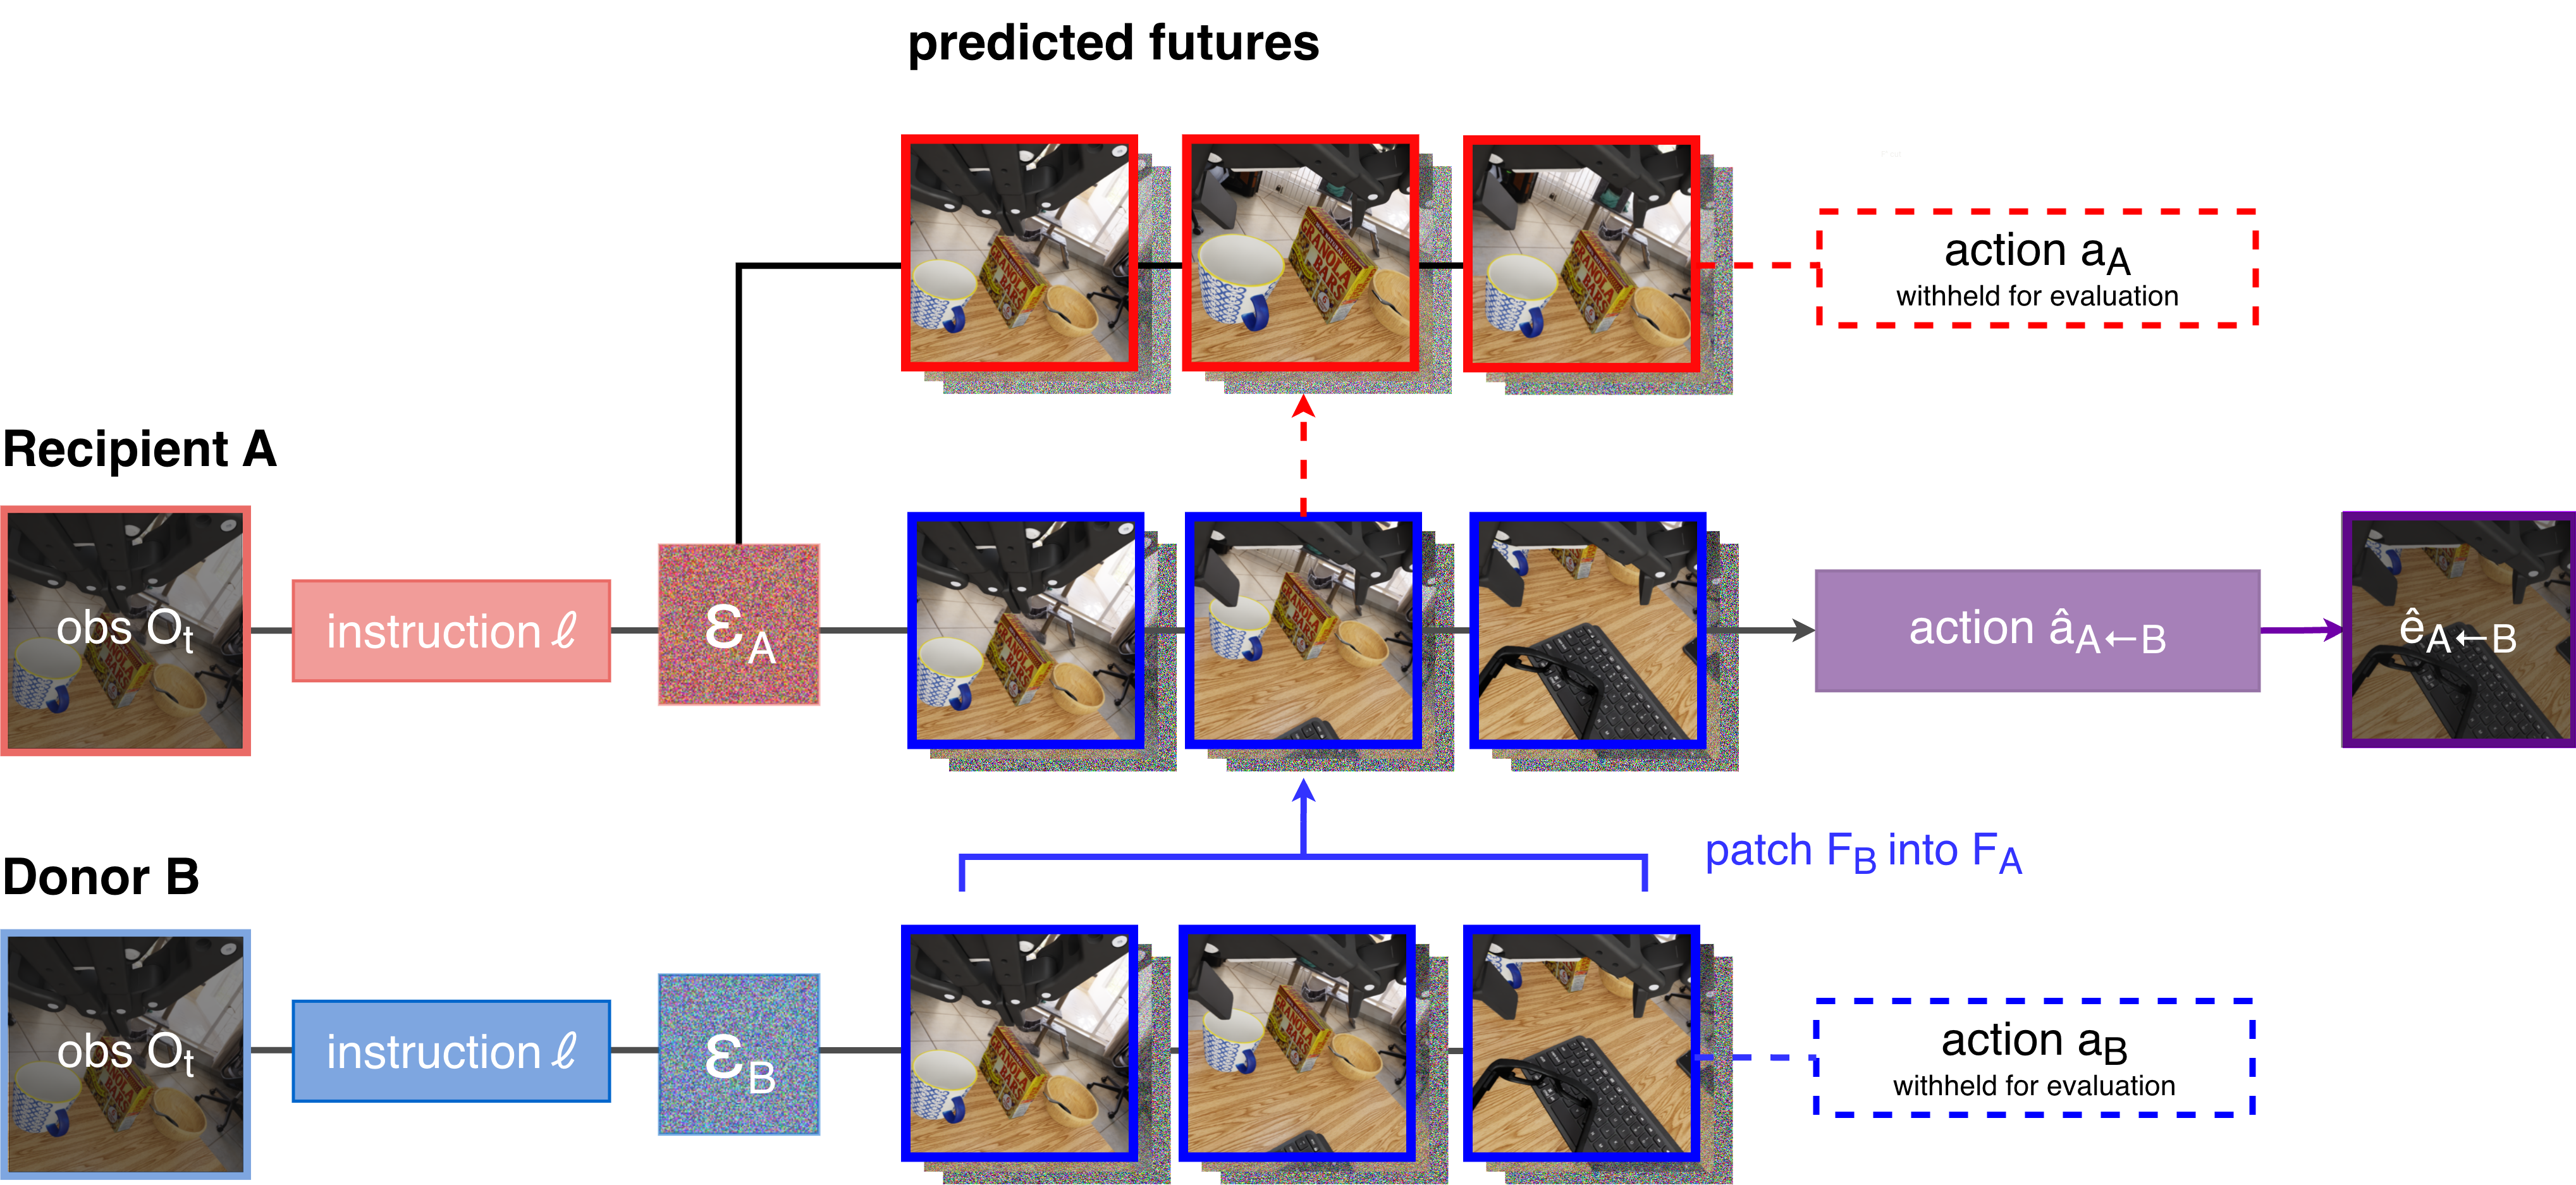
\includegraphics[width=0.96\textwidth]{figures/stage1_methodology.png}
  \caption{Future-content intervention. From two native rollouts at the same state, Stage 1 inserts donor $B$'s future target into recipient $A$ at every denoising step while holding the current observation fixed. We test whether the recomputed action and endpoint move toward $B$; the donor action is withheld and used only for evaluation. Cosmos Policy uses an executed-endpoint encoding; Cosmos 3 tests predicted latents and executed videos.}
  \label{fig:stage1_method}
\end{figure*}

\subsection{Stage 1: Future-content intervention}
\label{sec:stage1}

Starting from saved simulator state $S$, two unmodified rollouts produce recipient and donor futures $F_R,F_D$, actions $\mathbf a_R,\mathbf a_D$, and one-chunk endpoints $\mathbf e_R,\mathbf e_D$ (Figure~\ref{fig:stage1_method}). We restore $S$ and recompute the recipient while replacing only its future representation with $F_D$. Observation, instruction, recipient random draws, solver, denoising schedule, and action coordinates remain fixed. The donor target is reimposed at every denoising step. Cosmos Policy uses an encoding of proprioception and two camera views at the donor's executed endpoint; Cosmos 3 uses the donor's predicted video latent or an encoded video of its executed action. Appendix~\ref{app:future_replacement_impl} gives the exact mechanics.

For action or endpoint $\mathbf x\in\{\mathbf a,\mathbf e\}$, normalized donor projection is
\begin{equation}
\pi_x(\hat{\mathbf x};R,D)=
\frac{(\hat{\mathbf x}-\mathbf x_R)^\top(\mathbf x_D-\mathbf x_R)}
{\lVert\mathbf x_D-\mathbf x_R\rVert_2^2}.
\label{eq:projection}
\end{equation}
The recipient is 0 and donor is 1; changes orthogonal to the donor direction receive little weight. Steering subtracts the model-specific self reference. Every endpoint arm is executed after restoring the same state.

We evaluate \texttt{Cosmos-Policy-LIBERO-Predict2-2B} on ten LIBERO-Long tasks at the first query and after three and six open-loop chunks (30 registered states), and the 16B \texttt{Cosmos3-Nano-Policy-DROID} checkpoint on six RoboLab tasks (24 frozen state clusters; 22 completed) \citep{kim2026cosmospolicy,nvidia2026cosmospolicylibero,liu2023libero,nvidia2026cosmos3,nvidia2026cosmos3droid,yang2026robolab}. Pairs are selected by native action and endpoint separation, never intervention outcomes. Where applicable, self, matched-Gaussian, natural-alternative, shuffled-future, and bitwise no-op controls test recomputation, perturbation size, and generic replacement. State is the independent unit; repeated draws and reciprocal directions are averaged within state, with 10,000 state-bootstrap resamples. Full designs appear in Appendix~\ref{app:settings}--\ref{app:stage1_stats}.

\begin{figure}[H]
  \centering
  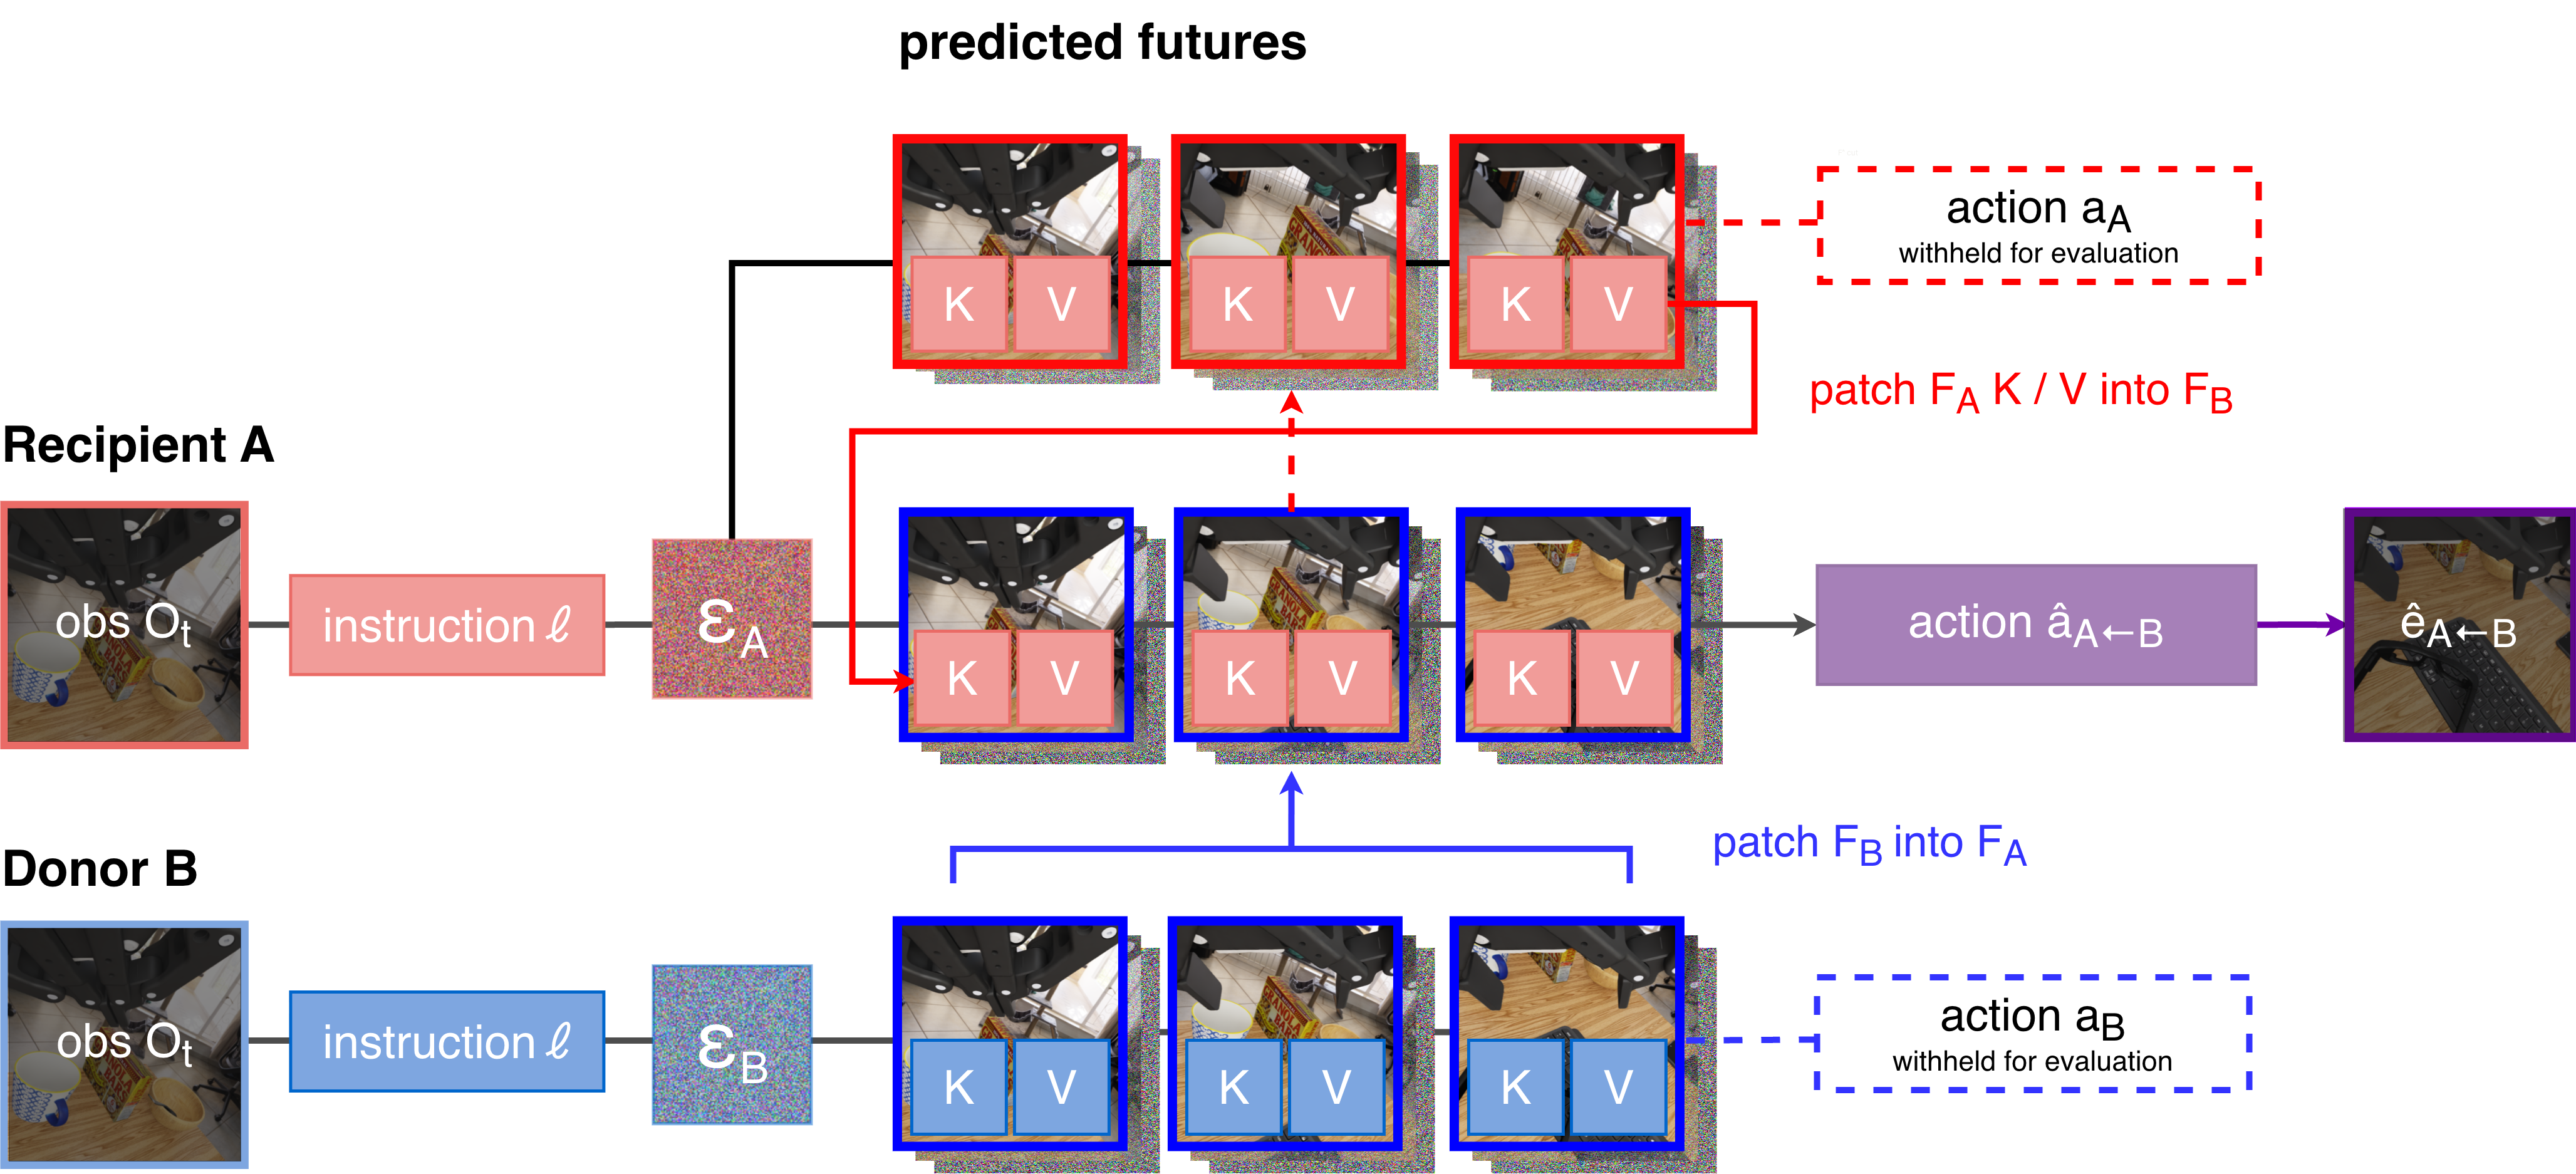
\includegraphics[width=0.96\textwidth]{figures/stage2_methodology.png}
  \caption{Stage-2 pathway intervention. The donor future remains inserted in recipient $A$, but predicted-future-position K/V is restored from $A$'s native run. The decrease in donor-directed steering measures how much of the Stage-1 effect passes through this interface.}
  \label{fig:stage2_method}
\end{figure}

\subsection{Stage 2: K/V pathway intervention}
\label{sec:stage2}

Stage 2 tests model-specific future-to-action attention routes. In Cosmos 3, we record K/V at predicted-future positions in the recipient's native run, leave $F_D$ inserted, and restore only those K/V states. The decrease in donor steering is \emph{K/V replacement loss}. Cosmos Policy removes future-position keys at a prespecified block.

For Cosmos 3, recipient K/V is recorded across all 36 layers and eight model forwards and replayed call by call during the donor-future run. Only action-query rows are recomputed; all other positions and states remain native to that run. The interface was selected on excluded calibration tasks and frozen before population testing. Cosmos Policy gates keys at predicted-future positions in prespecified block 27. Cache alignment, identity controls, calibration, and implementation details appear in Appendix~\ref{app:pathway_impl}.

\section{Results}
\label{sec:results}

\subsection{Coherent futures directionally steer behavior}
\label{sec:steering}

Across 22 Cosmos 3 states and all six tasks, the paired donor's predicted future produces action steering of $0.992$ ($[0.972,1.010]$; 22/22 states positive), versus $0.559$ for a naturally predicted alternative (Table~\ref{tab:directionality_short}). Executed donor videos produce action steering of $0.983$, compared with $0.591$ for the naturally predicted alternative and $0.041$ for the matched-Gaussian control. In secondary analyses, executing the recomputed action yields endpoint steering of $1.003$ ($[0.950,1.050]$; 22/22), versus $0.514$ and $-0.041$ for those controls. Thus, donor-directed change survives execution and is not explained by recomputation, an equally large unstructured displacement, or merely supplying a different valid prediction. Projection measures agreement along the donor direction, not equality of complete vectors.

At Cosmos Policy's first query, the paired donor produces action steering of $0.499$ and endpoint steering of $0.552$, positive in all ten tasks. Natural controls reach $0.395$ and $0.442$, shuffled controls $0.244$ and $0.275$, and Gaussian controls remain near zero. The paired donor exceeds the natural alternative by $0.103$ ($[0.048,0.161]$; 8/10) for actions and $0.110$ ($[0.054,0.166]$; 8/10) for endpoints. Steering is near zero at separately sampled later states, establishing state dependence rather than causal temporal decay.

\begin{table}[t]
  \caption{Stage-1 donor projections. Zero is the self reference and one is the native recipient-to-donor displacement. Intervals and state-level estimates appear in Appendix Figure~\ref{fig:directionality}.}
  \label{tab:directionality_short}
  \centering
  \scriptsize
  \setlength{\tabcolsep}{4.2pt}
  \begin{tabular}{@{}llrrrr@{}}
    \toprule
    Model & Outcome/source & Gaussian & Natural & Shuffled & Paired donor \\
    \midrule
    Cosmos 3 & Predicted action & --- & 0.559 & --- & \textbf{0.992} \\
             & Executed-video action & 0.041 & 0.591 & --- & \textbf{0.983} \\
             & Executed endpoint & $-0.041$ & 0.514 & --- & \textbf{1.003} \\
    \midrule
    Cosmos Policy & Action & 0.001 & 0.395 & 0.244 & \textbf{0.499} \\
                  & Executed endpoint & 0.003 & 0.442 & 0.275 & \textbf{0.552} \\
    \bottomrule
  \end{tabular}
\end{table}

\subsection{Content profiles differ across architectures}
\label{sec:content}

Cosmos Policy's early-state effect is concentrated in future visual inputs, especially the wrist-camera target. Wrist-camera replacement produces action steering of $0.435$ ($[0.284,0.605]$), primary-camera replacement $0.101$ ($[0.057,0.144]$), and future-proprioception replacement $0.001$ ($[-0.004,0.008]$). In a separate 20-state rendered-video study, the object-state main effect is approximately zero for action and endpoint, with decoder checks confirming that the imposed distinction remains visible. Across four exploratory natural-pair comparisons, robot-motion futures steer more strongly than object-motion futures, consistent with a role for camera-visible robot motion.

Cosmos 3 instead requires more than either isolated pixel factor. Across ten frozen factor-study states spanning all six tasks, a complete executed donor video strongly steers actions ($0.988$) and endpoints ($0.929$), but robot-pixel effects are $0.002$ and $0.010$ and object-pixel effects $0.006$ and approximately zero. Every isolated-factor interval lies within the prespecified $[-0.10,0.10]$ equivalence region. The effect may depend on distributed features or temporal and robot--object coherence. The result establishes factor insufficiency, not the irrelevance of robot or object information (Appendix Figure~\ref{fig:cosmos3_factorization}).

\subsection{Predicted-future K/V carries most Cosmos 3 steering}

Replacing K/V at predicted-future positions removes most of the Stage-1 effect (Table~\ref{tab:kv_short}). Predicted-action steering falls from $0.992$ to $0.115$, a loss of $0.877$ ($[0.842,0.910]$), or 88\%. Executed-action steering falls from $0.983$ to $0.169$, a loss of $0.814$ ($[0.723,0.900]$), or 83\%. Executed-endpoint steering falls from $1.003$ to $0.152$, a loss of $0.851$ ($[0.766,0.922]$), or 85\%. Loss is positive in all 22 states. Because the donor future remains inserted while positions and non-targeted states stay fixed, this identifies predicted-future K/V as a pathway carrying donor-specific influence. Nonzero residuals make the pathway influential but incomplete.

In Cosmos Policy, progressive key removal at block 27 produces a monotonic action-disruption curve. The absolute mean executed-endpoint projection change is $0.281$ ($[0.164,0.430]$; 10/10 states), exceeding equal-count random-key removal by $0.169$ ($[0.058,0.322]$; 9/10). This demonstrates sensitivity to future-position keys at block 27; current-key removal produces a statistically indistinguishable change.

\begin{table}[t]
  \centering
  \caption{Cosmos 3 K/V pathway test across 22 states. Replacement loss is the within-state decrease in donor steering; intervals are 95\% state-bootstrap intervals.}
  \label{tab:kv_short}
  \scriptsize
  \setlength{\tabcolsep}{5pt}
  \begin{tabular}{@{}lccc@{}}
    \toprule
    Outcome & Before & After & Loss [95\% CI] \\
    \midrule
    Predicted action & 0.992 & 0.115 & 0.877 [0.842, 0.910] \\
    Executed action & 0.983 & 0.169 & 0.814 [0.723, 0.900] \\
    Executed endpoint & 1.003 & 0.152 & 0.851 [0.766, 0.922] \\
    \bottomrule
  \end{tabular}
\end{table}

\section{Discussion and Limitations}

Controlled interventions turn an ambiguous co-generated output into testable claims about what changes behavior and how that effect is transmitted. Across both WAMs, the inserted future's identity predicts the direction of the resulting action and simulator endpoint. Cosmos Policy's early-state effect is concentrated in visual future targets, especially the wrist camera, whereas Cosmos 3's complete-video effect is not recreated by isolated robot or object pixels. Pathway tests show Cosmos Policy's sensitivity to future-position keys at block 27 and that K/V at predicted-future positions carries most of Cosmos 3's donor-directed shift.

This evidence remains narrower than planning. Planning would require generating alternatives, predicting their consequences, comparing them using a goal or value, and selecting among them. We do not test that sequence or establish stable success/failure mediation. The results instead show causal conditioning on coherent future content and identify one important internal route by which that content influences action.

\paragraph{Limitations.}
The main experiments evaluate two checkpoints in simulation across six RoboLab tasks and LIBERO-Long. They establish directional effects on actions and one-chunk endpoints rather than closed-loop task success. Pixel masks test localized visual factors, and the pathway interventions isolate specified attention interfaces rather than the entire circuit. Broader checkpoints and physical robots remain to be tested.

\paragraph{Responsible use.}
These methods could improve auditing by distinguishing visually plausible predictions from representations that actually control behavior. They could also redirect robot actions or encourage false confidence on narrow state distributions. Before physical deployment, mitigations should include broader coverage, independent replication, physical safety constraints, human oversight, and monitoring beyond the intervention metric.

\section{Conclusion}

Together, these interventions provide a causal framework for testing how specific imagined futures direct action and tracing their influence through future-token K/V.
